\section{Platform comparing}
In order to implement the previous discussed effects digitally, a platform has to be chosen. In this section a list of possible platforms for the effect implementation will be analysed. The following platforms will be analysed:

\begin{itemize}
\item Rasperry pi
\item \gls{dsp}
\item \gls{fpga}
\end{itemize}

The different platforms will be compared w.r.t \textbf{TBD}.

\subsection{Raspberry pi}
There exist different generations of the Raspberry pi, but the one that will be analysed is the Raspberry pi 3 model B, since it is the latest version. 
A Raspberry pi is a \gls{sbc} at the size of a credit-card. A picture of the Raspberry pi 3 model B, is shown in \autoref{fig:RP3mB}.

\begin{figure}[h]
	\centering
		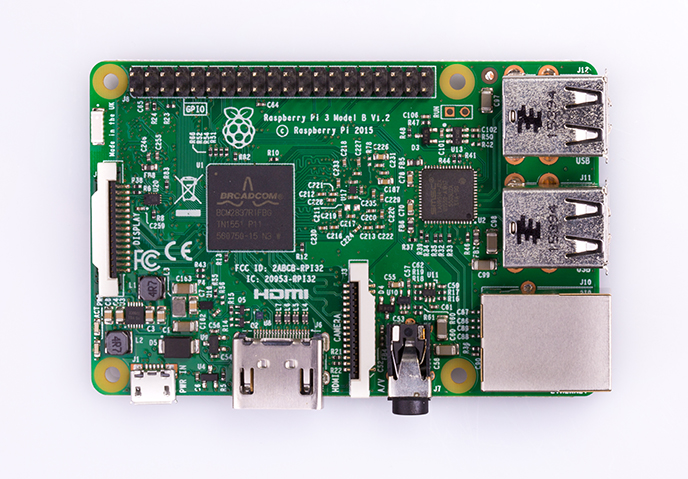
\includegraphics[width=0.7\textwidth]{Raspberry_pi_3_model_B.jpg}
		\caption{Picture of the Raspberry Pi 3 model B \cite{Rasperry_pi}.}
		\label{fig:RP3mB}
\end{figure}

The Raspberry pi 3 model B has a 1.2 GHz Quad-core ARM processor, supports wireless LAN and Bluetooth 4.1. It has 1GB RAM and has connectors for micro SD cards \cite{Raspberry_pi}.
The Raspberry Pi is Linux based, but can also run Windows \cite{sparkfun_Raspberry_pi}. This makes the Raspberry pi 3 model B suited for a wide range of projects. This is both its advantage and its disadvantage if a specialized platform is wanted. 

\subsection{Digital Signal Processor}
A \gls{dsp} is a processor, which is optimized for high-speed numerical operations such as: Addition, subtraction, multiplication and division. A typical \gls{dsp} system includes an anti-aliasing filter, an \gls{adc}, a \gls{dsp}, a host interface, a \gls{dac} and a anti-imaging filter. A block diagram of the typical \gls{dsp} system is shown in \autoref{}

\begin{figure}[h]
	\centering
		\begin{picture}(0,0)%

\includegraphics{document1.pdf}%
\end{picture}%
\setlength{\unitlength}{3947sp}%
\begingroup\makeatletter\ifx\SetFigFont\undefined%
\gdef\SetFigFont#1#2#3#4#5{%
  \reset@font\fontsize{#1}{#2pt}%
  \fontfamily{#3}\fontseries{#4}\fontshape{#5}%
  \selectfont}%
\fi\endgroup%
\begin{picture}(1062,1205)(2814,-3118) 
\put(3227,-2202){text}%
\end{picture}%
		\caption{Picture of the Raspberry Pi 3 model B \cite{Rasperry_pi}.}
		\label{fig:R}
\end{figure}